\documentclass[12pt, a4]{article}
\usepackage[utf8]{inputenc}
\usepackage{graphicx}
\usepackage{caption}
\usepackage{float}
\usepackage{listings}

\usepackage[utf8]{inputenc}
\usepackage[english]{babel}

\usepackage{biblatex}
\addbibresource{sample.bib}

\graphicspath{./imgs}

\lstset{
    language=C,
    aboveskip=3mm,
    belowskip=3mm,
    basicstyle={\medium\tttfamily},
    tabsize=4,
    numbers=left,
    captionpos=b,
    numbersep=8pt
}

\title{Problema de abastecimento à custo mínimo}
\author{Max William S. Filgueira e João Pedro de A. Paula}
\date{March 2019}

\begin{document}

\maketitle

\tableofcontents

\newpage

\section{Introdução do Problema}
\label{sec:intro}

A demanda incessante por produtos requer que fábricas por todo o mundo trabalhem
à todo vapor para supri-la e isto chama atenção ao problema associado a este o
qual não pode ser evitado: Como transportar adequadamente todos estes produtos?
Uma má estratégia de entregas resultaria em prejuízos para todos os envolvidos,
talvez seja mais caro enviar o mesmo caminhão para duas cidades em direções
opostas do que enviar um caminhão para cada cidade.

No contexto de grafos, as fábricas e as lojas são tratadas como vértices e as
arestas são as "estradas" entre as localizações de cada dois vertices.

\section{Modelagem do problema}
\label{sec:modelling}

Como mencionado na \ref{sec:intro}, cada vértice representa ou uma fábrica ou uma
loja, e as arestas entre cada dois vértices representariam um trajeto possível
entre as duas localizaçoes (uma "estrada"). Neste trabalho trataremos este como
um problema de fluxo à custo mínimo. Assim, serão necessárias algumas
modificações no grafo. A princípio, adicionaremos informações nas arestas, as
quais conterão os valores da capacidade mínimo e máxiao que pode percorrer esta
aresta e também um valor inteiro não-negativo associado ao custo de transporte
de uma unidade de um produto por esta estrada. Outro detalhe a ser corrigido é
que, para que os vértices sejam conservativos, precisamos garantir de alguma
maneira que o fluxo dos produtos ao chegarem em suas lojas "escorram" para algum
sumidouro, apesar de efetivamente os produtos permanecerem nas lojas. Assim,
cria-se uma aresta com custo 0 entre o vertice da loja e um novo sumidouro com
fluxo máximo igual à capacidade de estoque da loja, analogamente cria-se uma
fonte com arestas de peso 0 para os vértices de fábrica com fluxo mínimo e
máximo igual à produção da fábrica em questão. Todas as arestas entre vértices
que não são fonte nem sumidouro tem capacidade mínima igual a 0 e capacidade
máxima infinita.

\begin{figure}[H]
  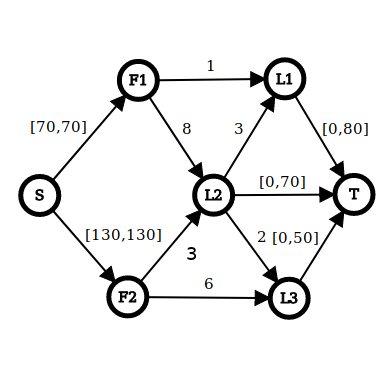
\includegraphics[width=\linewidth]{grafo.png}
  \caption{Um grafo modelado com o problema de fluxo a custo mínimo.}
  \label{fig:modeled-graph}
\end{figure}

\subsection{Estrutura do vértice}
\label{subsec:vertex-structure}

Dada a modelagem proposta, a estrutura dos vértices não difere da estrutura de
um vértice em um problema qualquer de grafos, visto que a informação vital
necessária para a solução do problema reside nas arestas, no mínimo seria
necessário que cada vértice armazenasse um id e os vértices adjacentes,
dependendo da forma de implementação.

\subsection{Arcos}
\label{subsec:arches}

Os arcos, sendo os portadores das informações essenciais para a solução deste
problema, possuem os valores das capacidades minimas e máximas das arestas (em
relação ao fluxo) e o valor do custo para transportar uma unidade do produto por
meio deles. Os arcos entre a fonte e as fábricas possuem capacidade mínima igual
à máxima, representativa da produção real da fábrica. Os arcos entre as lojas e
o sumidouro tem capacidade mínima 0 e a capacidade máxima representativa da
demanda real da loja. Todos os outros arcos tem capacidade mínima 0 e capacidade
máxima infinita.

\section{Estado da arte}
\label{sec:state-of-the-art}

\subsection{Minimum Mean Cycle-Cancelling}
\label{subsec:min-mean-cycle-cancelling}

A princípio, para cada aresta entre dois vertices $(u,v)$ cria-se uma aresta
$(v,u)$ com custo $c(v,u) = -c(u,v)$. Definimos o custo de um ciclo como a soma
dos pesos das arestas que o compõem. A ideia por trás deste algoritmo de
Goldberg e Tarjan é: se não houver nenhum ciclo na rede residual cujo custo for
negativo, então este fluxo é de custo mínimo.

Em teoria o algoritmo se resume em: encontre um ciclo de custo negativo, então
cancele ele aumentando o fluxo neste ciclo (saturando assim, ao menos uma
aresta), repita o processo até que não existam mais ciclos de custo negativo. De
forma semelhante ao algoritmo original de Ford e Fulkerson, dependendo da
magnitude do valor do fluxo, é possível que o algoritmo leve tempo exponencial
(e para valores irracionais ele pode nunca terminar). Devido a isto, definimos a
média de um ciclo como o custo do ciclo divido pela quantidade de arestas que o
compõem.

Podemos então repetir o procedimento já definido porém com base numa regra:
Buscando sempre o ciclo com menor custo, temos não só a garantia de termino do
algoritmo, como para grafos com arestas de peso inteiro o algoritmo tem
complexidade $O(mn \log(nC))$

\subsection{Network Simplex}
\label{subsec:network-simplex}

O algoritmo simplex mantém uma rede de fluxo viável a cada iteração. Uma solução
básica para o problema de fluxo à custo mínimo é denotado por uma tripla
$\langle T,L,U \rangle$, onde $T,L$ e $U$ são partições do conjunto de arcos.
$T$ é um conjunto de arcos básicos, isto é, arcos que fazem parte da árvore
geradora do grafo. $L$ e $U$ são respectivamente conjuntos com os arcos não
básicos nos seus limites inferiores e superiores. Nos referimos à tripla
$\langle T,L,U \rangle$ como uma \textit{estrutura básica} o fluxo $x$ associado
à estrutura básica da seguinte forma:

\begin{itemize}
\item Para cada arco $(u,v) \in U$: $x_{ij} = u_{ij}$.

\item Para cada arco $(u,v) \in L$: $x_{ij} = l_{ij}$.

\item Para os outros arcos, obtem-se valores quaisquer com a restrição apenas de
    que os vértices se mantenham conservativos.Dizemos que esta estrutura tem
    circulação viável se para todo arco de $T$ temos que
    $l_{ij} \leq x_{ij} \leq u_{ij}$.
\end{itemize}

Denotemos como $G^*(x)$ o subgrafo da rede residual $G(x)$ em relação ao fluxo
$x$ na qual todos os arcos da arvore geradora $T$ e seus arcos reversos foram
deletados. Isto é: $(u,v) \in G^*(x)$ se $(u,v) \in G(x)$ mas
$(v,u) \notin G(x)$.

Denotemos também uma arvore $T(v)$ como um subgrafo de $G(x)$ no qual todos os
arcos estão direcionados ao nó raiz $v$, tendo os custos e capacidades dos arcos
idênticos aos arcos definidos em $G(x)$.

Suponha que $x$ seja uma circulação básica viável, e seja $T$ a arvore geradora
associada. Se $(k,l) \in G^*(x)$, então o ciclo básico $W$ criado com a inserção
do arco $(k,l)$ em $T$ é a união de $(k,l)$ com o caminho pré-existente de $l$
até $k$ em $T(k)$. Um \textit{pivoteamento simplex} consiste em adicionar o arco
$(k,l)$ à arvore, enviar $\delta$ unidades de fluxo em $W$, e retira-se o arco
cuja capacidade residual foi reduzida para $0$ no processo (existe ao menos um).

Por último, definimos uma \textbf{condição ótima}. Uma estrutura básica
$\langle T,L,U \rangle$ é ótima se o custo de cada ciclo básico for não
negativo.

Assim, podemos definir o algoritmo em sua totalidade como abaixo:

\begin{figure}[H]
  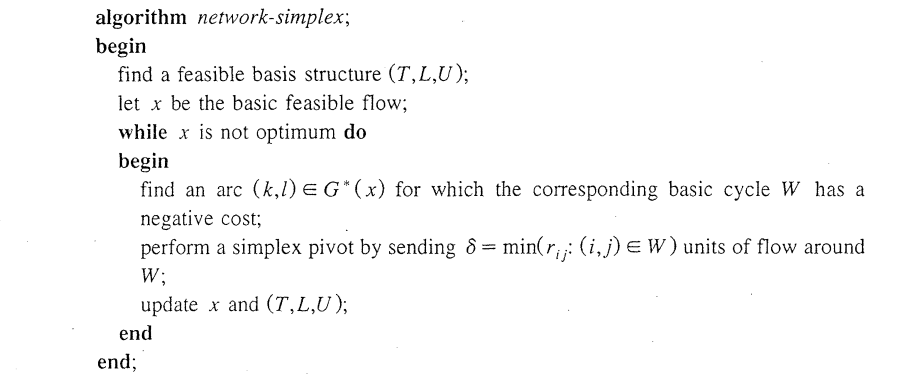
\includegraphics[width=\linewidth]{simplex.png}
  \caption{Algoritmo network simplex.}
  \label{fig:netwok-simplex-algorithm}
\end{figure}

\section{Menções importantes}
\label{sec:important-mentions}

Soluções para este problema cuja menção é indispensável encontram-se abaixo:

O algoritmo de Morton Klein utiliza-se de propriedades de programação linear,
mais especificamente caso a função de custo das arestas seja linearmente
convexa.

\begin{itemize}
\item Morton Klein (1967). "A primal method for minimal cost flows with
    applications to the assignment and transportation problems". Management
    Science. 14 (3): 205–220. CiteSeerX 10.1.1.228.7696.
    doi:10.1287/mnsc.14.3.205.
\end{itemize}

Algoritmo cuja solução proposta para o problema é acabar com todos os ciclos
negativos no grafo.

\begin{itemize}
\item Andrew V. Goldberg \& Robert E. Tarjan (1989). "Finding minimum-cost
    circulations by canceling negative cycles". Journal of the ACM. 36 (4):
    873–886. doi:10.1145/76359.76368.
\end{itemize}

Artigo com solução para o problema de fluxo à custo mínimo, mais especificamente
voltado para um subset deste, chamado assignment problem.

\begin{itemize}
\item Jack Edmonds \& Richard M. Karp (1972). "Theoretical improvements in
    algorithmic efficiency for network flow problems". Journal of the ACM. 19
    (2): 248–264. doi:10.1145/321694.321699.
\end{itemize}

Algoritmo de Goldberg e Tarjan que utiliza-se de programação linear e o conceito
de scaling para encontrar um algoritmo de complexidade O(n2(logn)log(nC)).

\begin{itemize}
\item Andrew V. Goldberg \& Robert E. Tarjan (1990). "Finding minimum-cost
circulations by successive approximation". Math. Oper. Res. 15 (3): 430–466.
doi:10.1287/moor.15.3.430.
\end{itemize}

Algoritmo network simplex, subset do algoritmo simplex clássico da programação
linear.

\begin{itemize}
\item James B. Orlin (1997). "A polynomial time primal network simplex algorithm
    for minimum cost flows". Mathematical Programming. 78 (2): 109–129.
    doi:10.1007/bf02614365. hdl:1721.1/2584.
\end{itemize}

\section{Solução escolhida}
\label{sec:solution}

\subsection{Dijkstra}
\label{subsec:dijkstra}

Como a busca em largura necessita que os pesos das arestas sejam 1, precisamos
utilizar um algoritmo de busca diferente para encontrar o menor caminho, visto
que dada modelagem do problema feita na seção \ref{sec:modelling} cada aresta
tem um peso associado, que se refere ao custo de transporte de um vértice ao
outro. O algoritmo escolhido para encontrar o menor caminho é o algoritmo de
Dijkstra.

O Dijkstra funciona da seguinte forma:

Chamemos o vértice de onde começamos de \emph{vértice inicial} e \emph{distância
    do nó $Y$} a distância entre o vértice inicial até o vértice $Y$. O
algoritmo atribui valores iniciais de distância e vai melhorando a cada
itereção, como segue:

\begin{enumerate}
\item Marque todos os vértices não visitados. Crie um conjunto de todos os
    vértices não visitados chamado \emph{conjunto não visitado} $Q$.
\item Atribua a cada vértice uma \emph{tentativa de distância}: atribua a zero
    para o nosso vértice inicial e infinito para todos os outros vértices. O
    vértice inicial será nosso \emph{vértice atual}.
\item Para o vértice atual $v$, considere todos os seus vizinhos não visitados
    $v' \in Q$ e calcule sua \emph{tentativa de distância} através do nó atual.
    Compare a nova \emph{tentativa de distância} com a atualmente atribuída e
    atribua a menor entre elas.
\item Após considerar todos os vizinhos do vértice atual $v$, marque o vértice
    atual como visitado e o remova do conjunto não visitado. Um vértice visitado
    nunca vai ser verificado novamente.
\item Se o vértice de destino $d$ tiver sido marcado como visitado, ou se a
    menor tentativa de distância entre os vértices do conjunto $Q$ for infinito,
    então pare. O algoritmo terminou.
\item Caso contrário, escolha o vértice $u$ do conjunto $Q$ de vértices não
    visitados que está marcado com a menor tentativa de distância; $u$ será o
    ``vértice atual''. Volte ao passo 3.
\end{enumerate}

A complexidade do algoritmo de Dijkstra é $O(m \log n + n)$, visto que visitamos
cada nó uma vez ($O(n)$) e acessamos cada vértice adjacente exatamente duas
vezes ($O(m)$), cada vez acessando a lista de prioridade no máximo duas vezes
($O(\log n)$).

\subsection{Edmonds e Karp}
\label{subsec:edmonds-karp}

A solução escolhida para o atual projeto é uma variante do algoritmo de
Ford-Fulkerson, o algoritmo de Edmonds e Karp, onde invés de utilizar um grafo
com arestas todas de peso 1, utilizamos arestas com o peso associado ao custo do
problema em questão. Durante a execução deste algoritmo, é criado um novo grafo
baseado no original, denominado de rede residual, onde os vértices são os mesmos
que os do grafo anterior, porém é composto apenas por arestas nas quais haviam
folga anteriormente (o fluxo que passava pela aresta era menor do que a
capacidade máxima da aresta). Uma das características principais do algoritmo de
Edmonds e Karp é que à cada iteração deste, é sempre encontrado o menor caminho
possível entre a fonte e o sumidouro da rede residual, por meio de uma busca em
largura. Entretanto, a busca em largura garante o menor caminho unicamente
quando o peso das arestas é igual a um. Assim, para encontra-lo é necessário o
uso de um algoritmo de menor caminho, como o Dijkstra por exemplo. Porém, como o
peso das arestas em questão era o custo associado de transporte do produto,
conseguimos a partir deste algoritmo o caminho de menor custo. Ao fim do
algoritmo teremos, por corretude do algoritmo de Edmonds e Karp, o fluxo
desejado na rede, e por meio da nossa escolha de caminhos de aumento de fluxo,
teremos que este fluxo será o de menor custo associado.

Analogamente ao algoritmo de Edmonds e Karp original, a complexidade deste
algoritmo é $O(nm) \times T(n,m)$ onde $T(n,m)$ é a complexidade do algoritmo de
menor caminho utilizado, $m$ é a quantidade de arestas e $n$ a quantidade de
vértices. A complexide $T(n,m)$ do algoritmo de Dijkstra implementado é
$O((m + n) \log n)$, visto que ele foi implementado com lista de adjacência e file de
prioridade,

Tomando como caso espécifico o algoritmo de Djikstra
temos $O(m^2 n + n^2 \log n)$.

\section{Conclusão}
\label{sec:conclusion}

Além de categorizar o problema de abastecimento entre fábricas e lojas como um
problema de fluxo à custo mínimo, apresentamos sua modelagem e algumas soluções
que podem resolvê-lo em tempo polinomial. Mostramos que podem ser diversas as
abordagens para o mesmo problema, enquanto uma variante de Edmonds e Karp
juntamente com o algoritmo de Dikstra pode ser o suficiente, este problema
também pode ser visto como um de programação linear, como no algoritmo simplex.

\end{document}

